%!TEX root = project.tex

\chapter*{About this project}
\paragraph{Abstract}
This project is an Social Media platform where you can create communities, post up discussions and follow your friends. . . .  etc etc

\paragraph{Authors}
Aaron Moran, Conor Shortt, Thomas Kenny.



\chapter{Introduction}
The final year project requires you to show initiative, consistency and the ability to showcase what you have learned over the course of four years.
Three members consist of Aaron Moran, Conor Shortt and Thomas Kenny. We are like minded students that share an interest for learning new skills and developing our ability as computer programmers. We have different skills that when combined complement each other from creativity to problem solving. With our interest in social media we decided early on that a social media website was a project that we felt we all could contribute too. A social media website requires multiple features, the in depth use of a database and an engaging UI. We were confident from the start with the team we have we could develop a website that could meet the standards of the websites out in the world today.
Before any developing took place, it was crucial we carried out in depth research into the top social media websites , how we were going to develop it , type of database to use and too draw up a timeline of goals/targets.



\newpage


\chapter{Context}
\begin{itemize}
\item Provide a context for your project.

\item Set out the objectives of the project
\item Briefly list each chapter / section and provide a 1-2 line description of what each section contains.
\item List the resource URL (GitHub address) for the project and provide a brief list of the main elements at the URL.
\end{itemize}

\section{Filler}


\chapter{Methodology}
About one to two pages.
Describe the way you went about your project:
\begin{itemize}
\item Agile / incremental and iterative approach to development. Planning, meetings.
\item What about validation and testing? Junit or some other framework.

For the development of this application, we decided the best approach to take was to use Agile. Agile is a methodology focused around iterative development. Using this method requires a team to work collaboratively and consistently. Before we started any development it was important to have a clear plan of what the features we wanted to incorporate and develop. Living in the same house proved useful in these times as we were able to have in-person meetings. Our first meeting we drew up a plan of how we were going to develop this application. Our first aim of was to agree on a development stack. After research into numerous development stacks such as the MEAN stack and MERN stack we decided on the MERN stack. Our research included ease of use , package management and plentiful of resources at our disposal. With our choice of stack agreed upon, the next step was dividing the roles in the group. Conor and Thomas have an interest in back-end development and Aaron was keen on developing the Front-end. The first meeting was beneficial as we had a concrete foundation to build upon. \newline
We decided the best approach to development was to work on two - three features a week. We set up a whiteboard with a list of features to be developed, every week we would divide the features between the three of us. An example of our work process is shown below.
===IMAGE OF WHITEBOARD===
Each week we would have a meeting detailing the work done and evaluate the features developed. This was an important process as we got to discover what we could improve and what works well. If something needed improving we would put it back on the list for future meetings. If a feature was functional and proved to be efficient we would cross it off the board. \newline
These meetings were also valuable for tracking bugs throughout the development process. If a team member encountered a bug or an issue we would write the it on the board and discuss it at the next meeting. Bug tracking was a process that requires good communication and teamwork as for an issue to be overcome we had to share solutions and potential bug fixes. 
\newline
Throughout the development of this project, we have used many collaboration tools including GitHub, Slack and Discord. While using these tools we were able to communicate new ideas and solutions to problems we may have been facing. GitHub helped us to track our progress and any mistakes that were made we could easily rollback commits. As we are all working on this project remotely, VOIP was incredibly important as we could communicate instantly, raising any issues we may be having and coming to brainstorming a solution.
\subsection{Testing}
Testing was a vital part of the development process. Using Agile required us to test after each feature was incorporated. We used many testing methods during the process of this application the two main testing methods used are White box testing and Black box testing.
\item Selection criteria for algorithms, languages, platforms and technolo-gies.
\end{itemize}
Check out the nice graphs in Figure \ref{tikz:graphs}, and the nice diagram in Figure \ref{tikz:mydiagram}.

\chapter{Experiments}
We tried out many of different experiments throughout the development of our project to improve its user experience and run-times. Between Front End and Back End we tried out many different design patterns and user interfaces that would suit our project and through trial and error found the best suitable solutions to suit our needs. We were able to utilize Googles lighthouse performance testing tool to examine our load times.
\newline

We faced issues while trying to load a large amount of images on a users feed and decided to experiment with ways around this bug. We tried reducing the amount of imported packages and keep the project package small so that it would be less pressure on the website when running. This clean up didn't seem to make any improvements on our website speeds and load times, but was still a successful experiment as it tidied up our code and removed any unnecessary and unwanted external packages.
\newline

We then attempted reducing the amount of shared information between collections within our MongoDB database, instead of passing all of the posting users information we only shared the ID keys which would give us full access to the details of the posting user and the posts information. Changing this structure within the communication between our collections saved us many resources and storage space within our database. This only marginally improved load times but was a success as it made our website perform at a higher speed than previously, and we learned a new solution to sharing information within our application which could be applied to many other features and functionalities.
\newline

AMAZON SOLUTION HERE
\newline

\begin{itemize}
    \item Website Runtimes
    \item Responsiveness
    \item Speeds and Performance
    \item Loaing in images via MongoDB/Amazon
\end{itemize}


\begin{itemize}
    \item Front End
    \item Colorways
    \item UI
    \item FIGMA, WIREFRAME
    \item Design Decisions
    \item Icon imports, Boostrapping
\end{itemize}

Throughout the development of this project we tried out many different User Interfaces and Front-End designs to try and find which was the most suitable layout for our project. We used software such as Figma and Wireframing to design and test our designs which we could implement, once we had three official designs we came to a conclusion on which one would be most suitable for our project to match its features.

\chapter{Results}

\chapter{Conclusion}
Ultimately, working as a team to develop this project etc etc ...


\begin{figure}
  \centering
  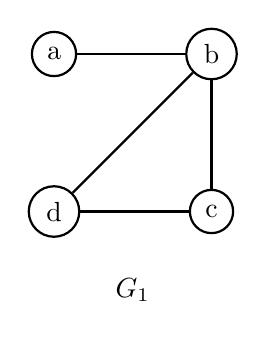
\begin{tikzpicture}
  \begin{scope}[every node/.style={circle,thick,draw}]
  \node (a) at (0,2) {a};
  \node (b) at (2,2) {b};
  \node (c) at (2,0) {c};
  \node (d) at (0,0) {d};
  \end{scope}
  \begin{scope}[every edge/.style={draw=black,thick}]
  \path (a) edge (b);
  \path (b) edge (c);
  \path (b) edge (d);
  \path (c) edge (d);
  \end{scope}
  \node () at (1,-1) {$G_1$};
  \end{tikzpicture}
  \hspace{1.5cm}
  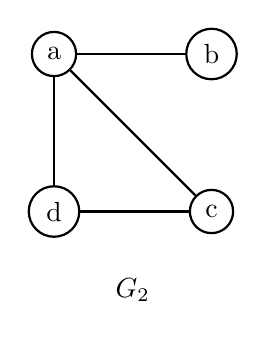
\begin{tikzpicture}
  \begin{scope}[every node/.style={circle,thick,draw}]
  \node (1) at (0,2) {a};
  \node (2) at (2,2) {b};
  \node (3) at (2,0) {c};
  \node (4) at (0,0) {d};
  \end{scope}
  \begin{scope}[every edge/.style={draw=black,thick}]
  \path (1) edge (2);
  \path (1) edge (3);
  \path (1) edge (4);
  \path (3) edge (4);
  \end{scope}
  \node () at (1,-1) {$G_2$};
  \end{tikzpicture}
  \caption{Nice pictures}
  \label{tikz:graphs}
\end{figure}


\begin{figure}
  \centering
  \begin{tikzpicture}[node distance=6cm]
  \node (a) [rect] {A Big Blue Block};
  \node (b) [oval, right of=a] {And His Oval Friend};
  \draw [line] (a) -- (b);
  \end{tikzpicture}
  \caption{Nice pictures}
  \label{tikz:graphs}
\end{figure}


\chapter{Technology Review}
About seven to ten pages.
\begin{itemize}
\item Describe each of the technologies you used at a conceptual level. Standards, Database Model (e.g. MongoDB, CouchDB), XMl, WSDL, JSON, JAXP.
The development stack we have chosen is the MERN stack, this consists of MongoDB, ExpressJS, ReactJS and NodeJS. The reason as to why we chose this development stack is because it can be easily divided up between Front-End and Back-End. Although we cross collaborated on both sections and helped each other whenever we were facing any issues, it was easiest to give each team member a main focus. Aaron worked mostly on the Front-End and Thomas and Conor worked together on the Back-End.


\item Use references (IEEE format, e.g. [1]), Books, Papers, URLs (timestamp) – sources should be authoritative. 
\end{itemize}

\section{XML}
Here's some nicely formatted XML:
\begin{minted}{xml}
<this>
  <looks lookswhat="good">
    Good
  </looks>
</this>
\end{minted}

\chapter{System Design}
As many pages as needed.
\begin{itemize}
\item Architecture, UML etc. An overview of the different components of the system. Diagrams etc… Screen shots etc.
\end{itemize}

\begin{table}[h]
  \centering
  \begin{tabular}{x{2cm}p{3cm}}
    \toprule \\
    Column 1 & Column 2 \\
    \midrule \\
    Rows 2.1 & Row 2.2 \\
    \bottomrule
  \end{tabular}
  \caption{A table.}
  \label{table:mytable}
\end{table}

\chapter{System Evaluation}
As many pages as needed.
\begin{itemize}
\item Prove that your software is robust. How? Testing etc. 
\item Use performance benchmarks (space and time) if algorithmic.
\item Measure the outcomes / outputs of your system / software against the objectives from the Introduction.
\item Highlight any limitations or opportuni-ties in your approach or technologies used.
\end{itemize}

\chapter{Conclusion}
About three pages.

\begin{itemize}
\item Briefly summarise your context and ob-jectives (a few lines).
\item Highlight your findings from the evalua-tion section / chapter and any opportuni-ties identified.
\end{itemize}

